
\chapter{Implementierung}
\label{chapter-implementierung}
Das folgende Kapitel beschreibt die Implementierung des Reservierungsinterfaces
sowie des Frontends. Zunächst wird die Implementierung des
Reservierungsinterfaces und die damit einhergehenden technischen Aspekte
beschrieben. Dabei wird Aufschluss über die Struktur gegeben und die
Kernfunktionalitäten sowie Sackgassen\todo{ugs.? herausforderungen? oder kursiv}
in der Realisierung näher erläutert. Daraufhin wird die Umsetzung des
Frontends erläutert. Abschließend wird auf die Inbetriebnahme des Systems
eingegangen.


\section{Implementierung des Reservierungsinterfaces}
Dieser Abschnitt erläutert den technischen Aufbau des Rervierungsinterfaces und
geht auf relevante Aspekte in der Realisierung der Kernfunktionalitäten
(\ref{section:funktionale}) ein. Des Weiteren werden unerwartete
Herausforderungen thematisiert, welche im Rahmen der Arbeit nicht bewältigt
werden konnten.


\subsection{Aufbau des Reservierungsinterface}
Das Reservierungsinterface teilt sich in drei wesentliche Bestandteile:
der \textit{Fastify-HTTP-Server}, die \textit{SQLite Datenbank} und das \textit{ORM
  Prisma} (vgl. \ref{fig:level3}). Diese Komponenten spiegeln sich auch in der Verzeichnisstruktur aus \ref{fig:db} wider.

\begin{figure}[h]
  \centering
  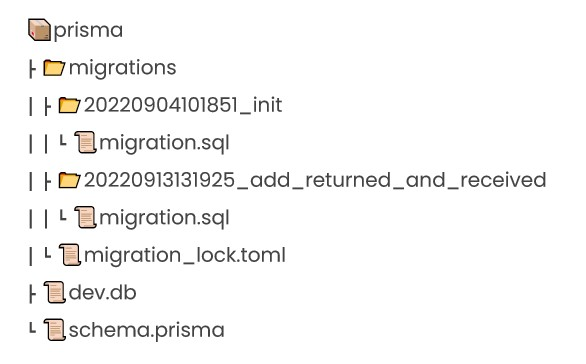
\includegraphics[scale=0.7]{Bilder/Db.jpg}
  \caption[Verzeichnisstruktur des Reservierungsinterfaces]{Verzeichnisstruktur des Reservierungsinterfaces}
  \label{fig:db}
\end{figure}

Der HTTP-Server findet sich in der \textit{server.ts} wieder und stellt dort die
API des Reservierungsinterfaces bereit. Die entwickelte API lässt sich in drei
Bereiche teilen: \textit{Assets}, \textit{Kategorien} und
\textit{Reservierungen} (\ref{table:impl-backend-routes}). Für die drei
Inhaltstypen werden die Routen aus \ref{table:impl-backend-routes}
bereitgestellt, welche die von \citeA{fielding_hypertext_2014} beschriebene
Semantik für HTTP-Methoden beachten. Folglich werden bei Verwendung der
\textit{GET}-Methode ausschließlich Daten zurückerhalten. Hingegen muss bei
einer Anfrage mit zu übermittelnden Daten die \textit{POST}-Methode verwendet
werden, um einen neuen Eintrag im System zu erschaffen. Beispielsweise wird eine
\textit{GET}-Anfrage an \textit{/assets/:id} abgeschickt, um die Informationen
eines Assets zu erhalten. Um den Status in Snipe-IT auf \textit{herausgegeben}
zu aktualisieren, wird eine \textit{POST}-Anfrage an
\textit{/reservation/receive} gesendet, sobald Verleihende eine abgeholte
Reservierung bestätigen.

\begin{table}[h]
  \centering
  \caption{API des Reservierungsinterfaces}
  \begin{tabular}{lll}
    \arrayrulecolor{maincolor}\hline
    \sffamily\color{maincolor}Methode & \sffamily\color{maincolor}Route &
    \sffamily\color{maincolor}Funktion
    \\
    \arrayrulecolor{maincolor}\hline
    GET                               & \textit{/assets}                &
    Erhalte alle Assets                                                   \\
    GET                               & \textit{/assets/:id}            &
    Erhalte ein Asset mit der entsprechende ID                            \\
    GET                               & \textit{/categories}            &
    Erhalte alle Kategorien                                               \\
    GET                               & \textit{/reservation}           &
    Erhalte Reservierungen                                                \\
    POST                              & \textit{/reservation}           &
    Erstellen Reservierung                                                \\
    POST                              & \textit{/reservation/receive}   &
    Erstellen Reservierung                                                \\
    POST                              & \textit{/reservation/return}    &
    Erstellen Reservierung                                                \\
    POST                              & \textit{/reservation/id}        &
    Erstellen Erstellen Reservierung                                      \\
    DELETE                            & \textit{/reservation/delete}    &
    Löschen Reservierungen                                                \\
    PATCH                             & \textit{/reservation/patch}     &
    Verändern Reservierung                                                \\
    \arrayrulecolor{maincolor}\hline
  \end{tabular}
  \label{table:impl-backend-routes}
\end{table}

Die mit SQLite bereitgestellte Datenbank speichert die Reservierungen sowie die
Nutzenden. Hierfür wurde das in \ref{fig:orm} dargestellte Datenbankschema
erarbeitet. Zur Umsetzung dieses Schemas wurde das ORM Prisma genutzt, welches
drei zentrale Aufgaben vereinfacht.

\begin{enumerate}[1]
  \item Schema: Die in einer Datenbank zu erstellenden Anforderungen werden
        durch Prisma in vielerlei Hinsicht abgenommen. Das zu erstellende Schema
        benötigt keine SQL-??. Um die Datenbanken (User und Reservation) erstellen zu
        können werden keinerlei Befehle benötigt, dies geschieht ebenfalls über
        Prisma. Folglich ist das Schema entsprechend vereinfacht (\ref{fig:prisma}).
  \item .
  \item .
\end{enumerate}

\begin{lstlisting}[style=pseudo,gobble=2,caption={Pseudocode: Kategorien anzeigen},label=fig:prisma]
    // This is your Prisma schema file, learn more about it in the docs: https://pris.ly/d/prisma-schema

        generator client {
          provider = "prisma-client-js"
        }

        datasource db {
          provider = "sqlite"
          url      = env("DATABASE_URL")
        }

        model User {
          id           Int           @id @default(autoincrement())
          email        String        @unique
          name         String?
          reservations Reservation[]
        }

        model Reservation {
          id        Int      @id @default(autoincrement())
          assetId   Int
          dateStart DateTime
          dateEnd   DateTime
          User      User     @relation(fields: [userId], references: [id])
          userId    Int
          received  Boolean  @default(false)
          returned  Boolean  @default(false)
        }
\end{lstlisting}


Ergänzt wird diese durch das ORM Prisma.
stellt die mit \textit{prisma} entwickelte Datenbank als Object Relational
Mapper (ORM) mit folgendem Schema dar. \textit{User} können
\textit{Reservierungen} aufgeben.

\begin{figure}[h]
  \centering
  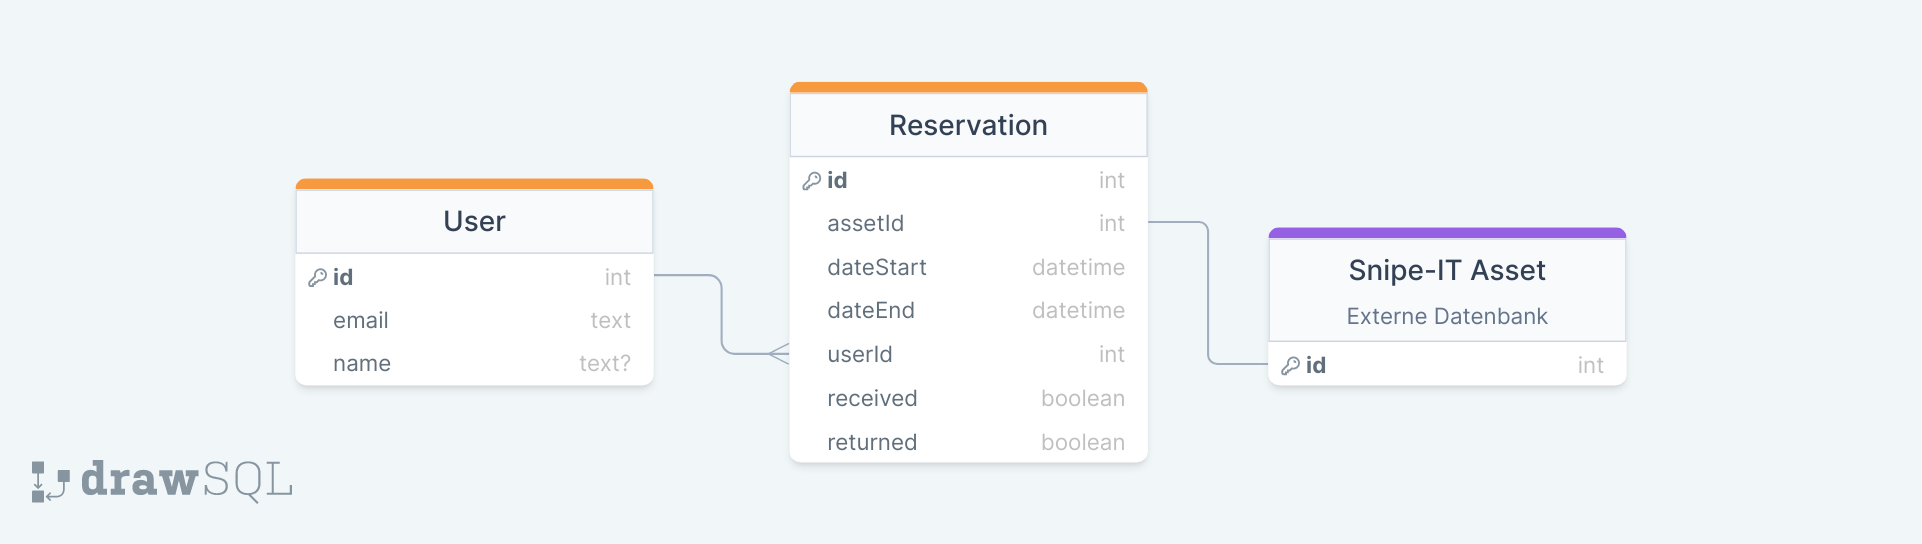
\includegraphics[scale=0.2]{Bilder/drawSQL-export-2022-10-09_15 56.png}
  \caption[Datenstruktur der Reservierungen in Verbindung mit Nutzenden]{Datenstruktur der Reservierungen in Verbindung mit Nutzenden}
  \label{fig:orm}
\end{figure}


\subsection{Implementierung der Kernfunktionalität} \todo{vielleicht Probleme in einem Kapitel
  Zweiter Ordnung am Ende des Implementierungskapitels zusammen, das wäre insgesamt stimmiger? }
  Dieser Abschnitt präsentiert die Implementierung der Kernfunktionalität des
  Reservierungsinterfaces, welche aus den Anforderungen bestimmt wurden (\ref{section:anforderung}).
  Bei der Funktionalität handelt es sich um das Reservieren in die Zukunft, sowie das Speichern
  dieser Vorgänge und die damit einhergehende Bestätigung für die Aktualisierung in Snipe-IT.
  Konkret wird auf das LDAP-System und das Reservieren von Assts eingegangen.

Um auf die Assets zugreifen zu können, wurde mit der Snipe-IT JSON REST API
gearbeitet. Die Snipe-IT API umfasst viele Ressourcen. Relevante Ressourcen für
die Umsetzung der Arbeit waren \textit{/hardware, /statuslabels, /users,
  /categories}. Mithilfe dieser konnten die Assets der Beispieldatenbank verwendet
werden. \ref{fig:snipe} zeigt die Beziehungen der API, beispielsweise ist ein
\textit{/statuslabel} immer an einen \textit{/user} gebunden.

\begin{figure}[h]
  \centering
  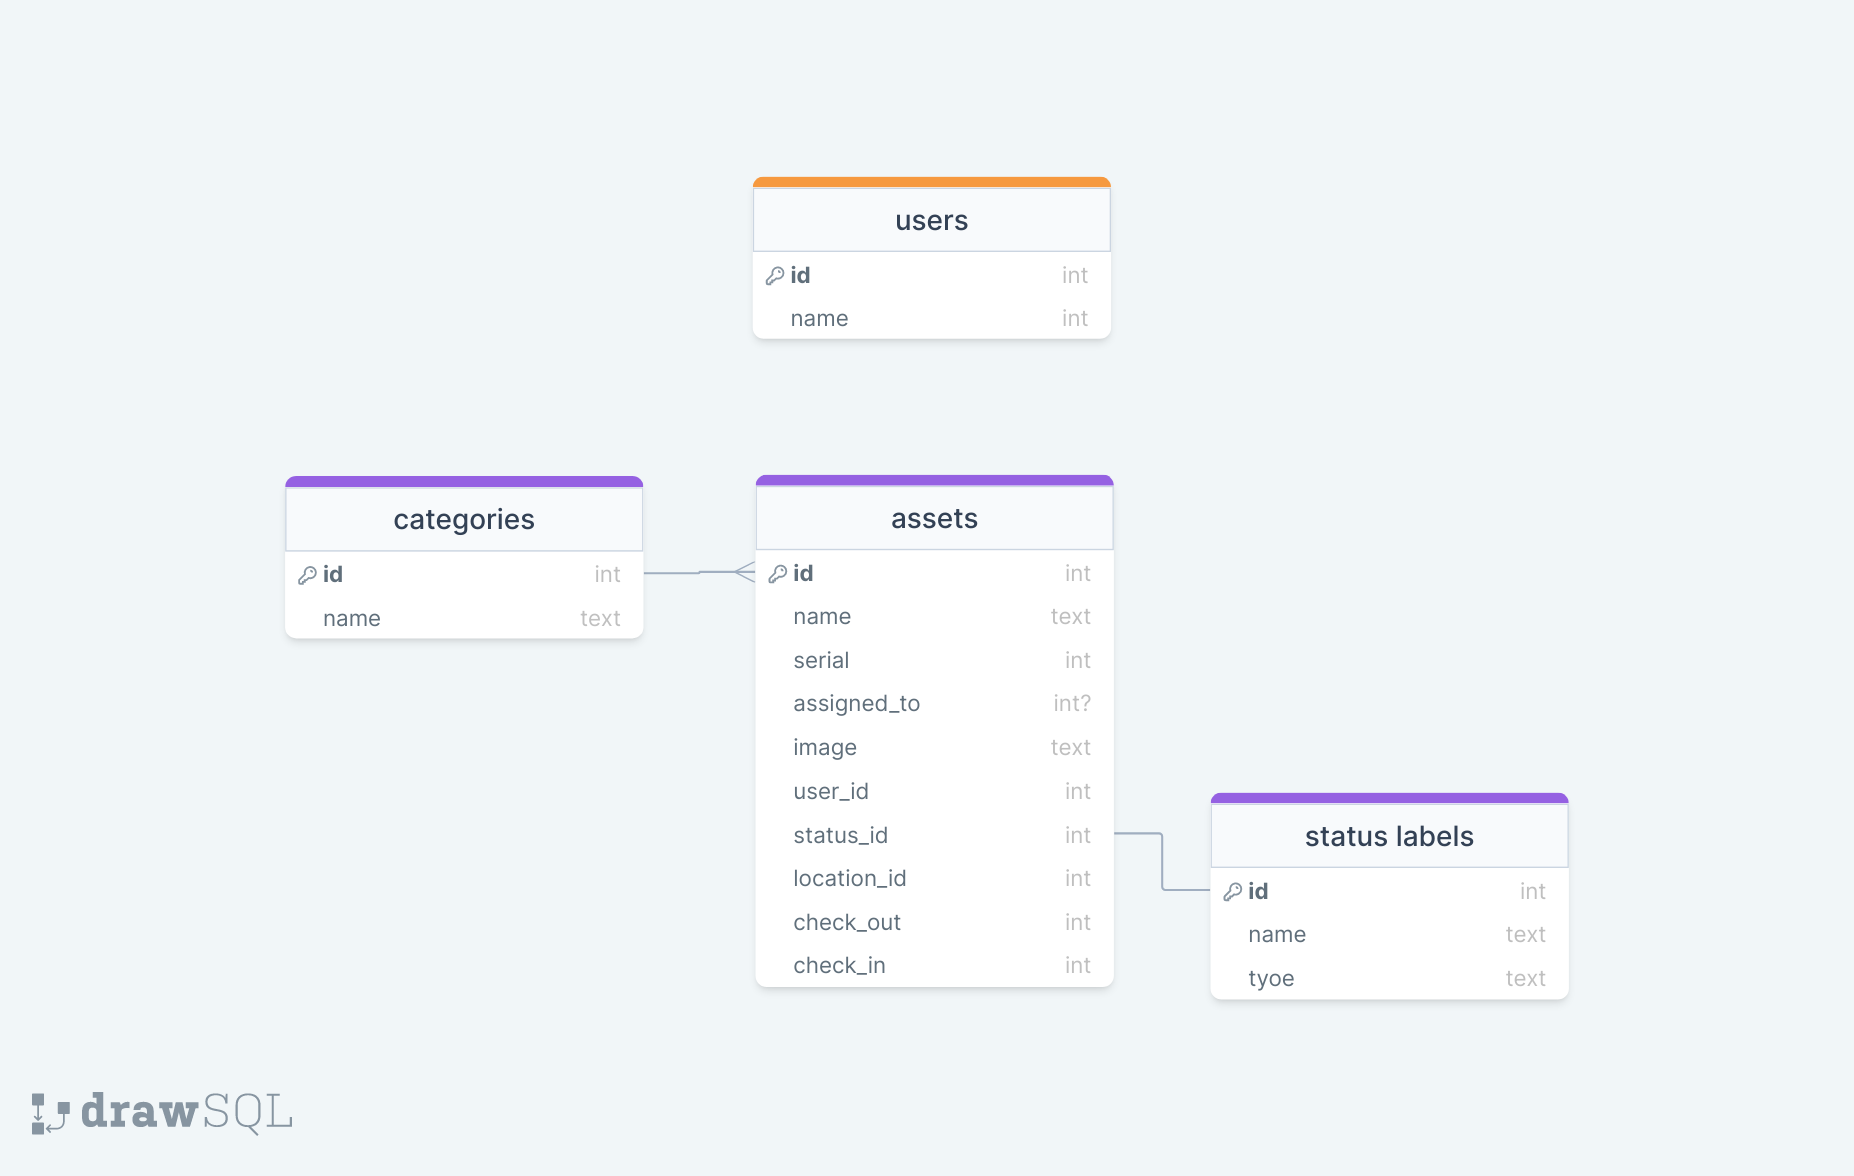
\includegraphics[scale=0.2]{Bilder/drawSQL-export-2022-10-12_17 27.png}
  \caption[UML Snipe-IT API]{UML Snipe-IT API}
  \label{fig:snipe}
\end{figure}

Um mit der API arbeiten zu können muss ein \textit{API
  key}\footnote{\url{https://snipe-it.readme.io/reference/generating-API-tokens}}
generiert werden. Da persönliche Zugriffstoken verwendet werden, spiegeln die
Berechtigungen des API-Tokens die Berechtigungen des Nutzenden wider. Das
bedeutet, dass die Token lediglich manuell im Dashboard generierbar sind. Was
zur Folge hat, dass das geplante LDAP-System der Universität zu Lübeck nicht
ohne Umstände eingebunden und entsprechend genutzt werden kann. Snipe-IT gibt
unter anderem die Möglichkeit, das LDAP
Formular\footnote{\url{https://snipe-it.readme.io/docs/ldap-sync-login}}
simpel einzubinden, trotz dessen besteht das Problem der Authentifizierung
sowie Generierung der Tokens, da die Daten im Reservierungsinterface bis dato
nicht übertragen werden können. Dies führt zu einem Datenschutzproblem.


Um unter anderem ein besseres Verständnis der Interaktion von einzelnen
Komponenten voraussetzen zu können, wurde ein UML-Sequenzdiagramm erstellt
(\ref{fig:uml}). Bei der vierten Komponente handelt es sich um das LDAP-System
der Universität zu Lübeck. Mithilfe der Integration können Nutzende sich mit
ihrem bereits bestehenden IDM Account anmelden. Zum einen kann somit
sichergestellt werden, dass nur befugte Personen Assets einsehen und ausleihen
können. Zum anderen erleichtert es den Nutzenden den Ausleihprozess, da kein
neuer Account erstellt werden muss.

\begin{figure}[h]
  \centering
  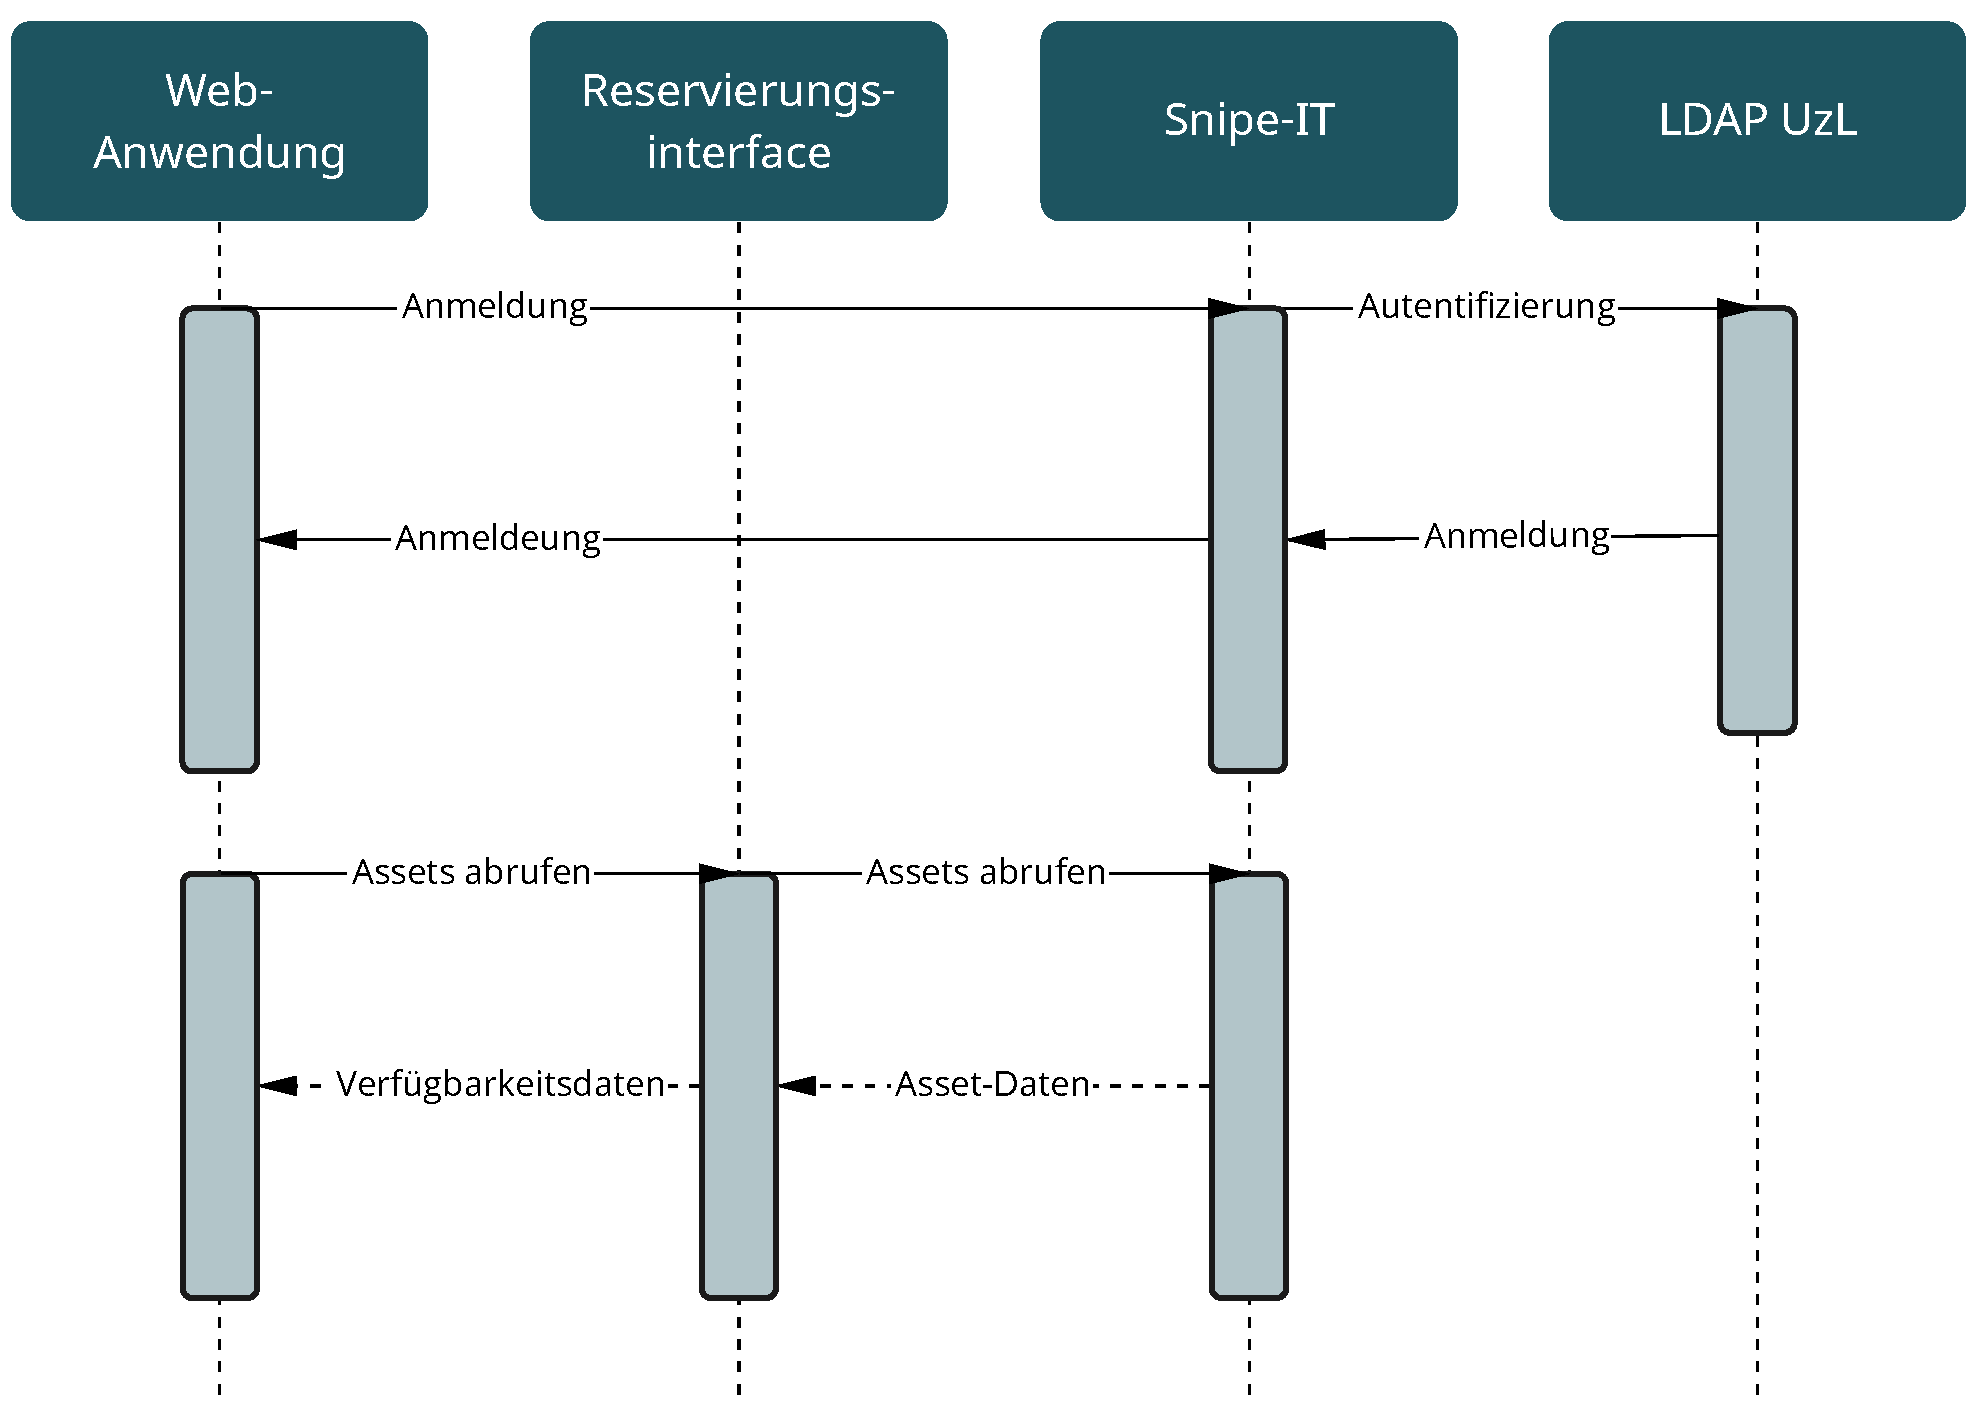
\includegraphics[scale=0.45]{Bilder/uml.pdf}
  \caption[UML-Sequenzdiagramm]{UML-Sequenzdiagramm}
  \label{fig:uml}
\end{figure}

Die für das Frontend benötigten Ressourcen wurden über den angelegten Routen
erstellt. Zur Unterstützung wurde \textit{Fastify} verwendet. \textit{Fastify}
ist ein Webframework für \textit{Node.js}. Das Framework verfügt über vielerlei
Plugins und ist daher gut erweiterbar, außerdem erleichter es DINGE.

Der eigentliche Kern der Anwendung befasst sich mit dem Reservieren der Assets.
Hierfür müssen die Daten (Assetname, Datum, Uhrzeit, Ort, \dots) gespeichert
werden. Bevor ein Status eines Assets in Snipe-IT von \textit{ausleihbar} zu
\textit{herausgegeben} geändert wird, werden die Daten für eine Reservierung im
Reservierungsinterfaces zwischengespeichert. Für diesen Schritt wurde SQLite
verwendet. Zusätzlich wurde für eine leichtere Verwaltung der angelegten
Datenbank Prisma genutzt. Die von Snipe-IT zur Verfügung gestellten
Möglichkeiten der Statuseingabe/Ausleihen schwer und komisch -> rumarbeiten.

\todo[inline]{Gibt es sonst etwas Wichtiges, was man hier erwähnen sollte? Code Beispiele?}

\section{Implementierung des Frontends} \todo{Verweis auf die Dokumentationen,
  Hier unbedingt Rückbezug auf Konzeption nehmen} Das kommende Unterkapitel
beschreibt die Client-seitige Realisierung der Arbeit. Zunächst wird der
Aufbau betrachtet (\ref{fig:vue}), daraufhin wird die Nutzung von vue und XXX
erläutert. Des Weiteren wird auf die Struktur der Komponenten eingegangen
(\ref{fig:komponenten}). Abschließend wird das native App-Erlebnis
thematisiert.

\begin{figure}[h]
  \centering
  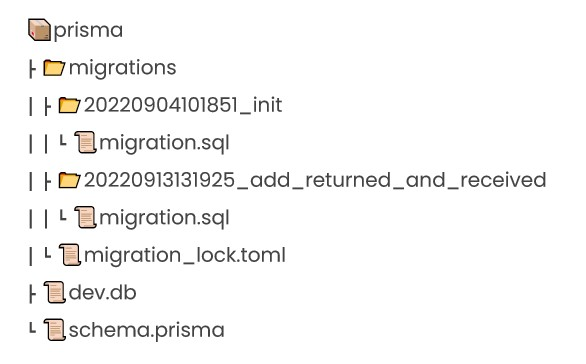
\includegraphics[scale=0.7]{Bilder/Db.jpg}
  \caption[Verzeichnisstruktur des Reservierungsinterfaces]{Verzeichnisstruktur des Reservierungsinterfaces}
  \label{fig:vue}
\end{figure}

Für den Aufbau des Projektes wurde aus den in \ref{chapter-konzept}
festgestellten Anforderungen \textit{vue.js} verwendet. Bei der Implementierung
wurde sich an den best practices der Vue.js-Dokumentation orientiert
\todo{(Vue.js, 2021a)}. Für sich wiederholende Elemente wurden eigene Views
erstellt. Dadurch ergibt sich eine hierarchisch geschachtelte Client-Anwendung
der Vue-Komponenten. \ref{fig:Komponenten} stellt die Komponenten-Struktur
vereinfacht dar. Um konkretere Vorschläge in der Entwicklungsumgebung zu
ermöglichen und vorzeitige Fehler zu minimieren, wurde ergänzt zu
\textit{JavaScript} \textit{TypeScript} verwendet.

\begin{figure}[h]
  \centering
  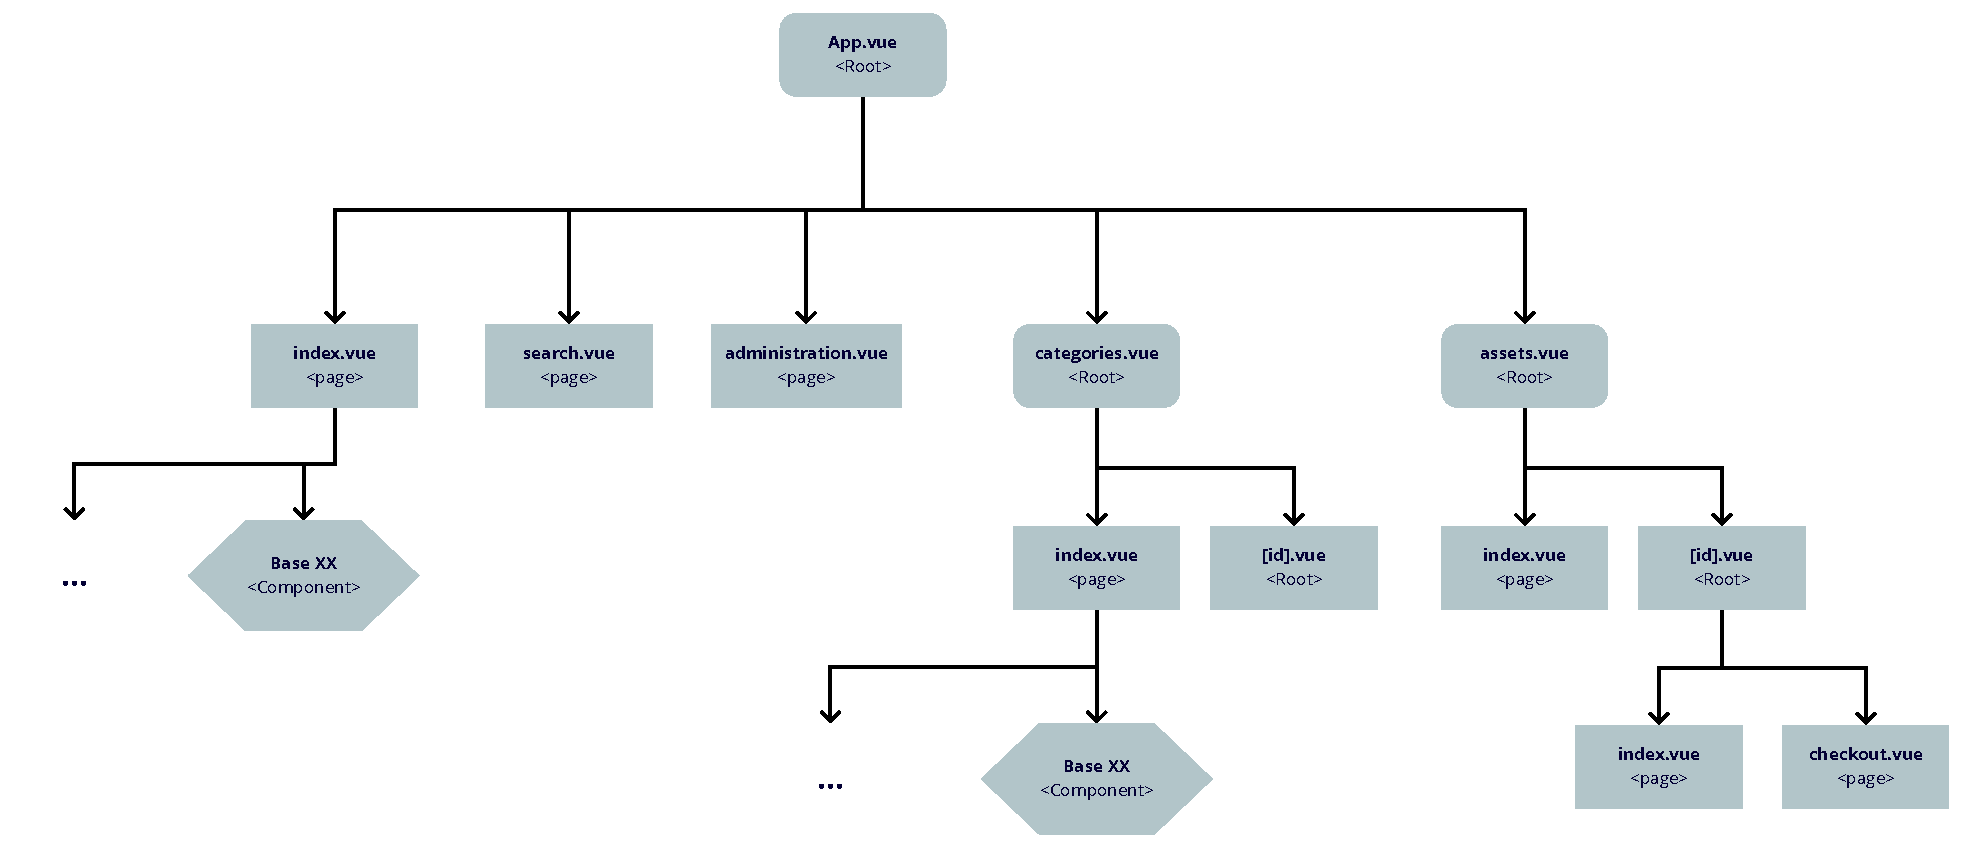
\includegraphics[scale=0.5]{Bilder/struktur.pdf}
  \caption[Vereinfachte Struktur der Komponenten]{Vereinfachte Struktur der Komponenten}
  \label{fig:Komponenten}
\end{figure}

Um das Styling zu vereinfachen wurde \textit{Tailwindcss} genutzt. Ergänzend
dazu wurde \textit{Preline} für UI verwendet. -> Nicht empfehlenswert
(Sackgassen). Für Animationen und Transitionen wurde \textit{HeadlessUi}
genutzt.

Der Kalender stellt einen wichtigen Bestandteil für das Reservieren von Assets
dar. Die Kalenderkomponente wurde durch \textit{v-calender} ergänzt. Durch die
Möglichkeiten der Komponente ...??. Außerdem bietet diese viele
Ausbaumöglichkeiten für folgende Funktionalitäten.

Die im Rahmen dieser Arbeit verwendete Beispieldatenbank beinhaltete eine
Vielzahl an Kategorien und Unterkategorien, welche wie folgt, eingetragen wurde:
\enquote{Kategorie - Unterkategorie}. Da das Anzeigen von den Kategorien
unübersichtlich ist, sollten zunächst nur die Kategorien und dann die
Unterkategorien angezeigt werden. \ref{fig:categoriecode} stellt den
Entwickelten Algorithmus als Pseudocode dar. Der \enquote*{-} wurde dazu als
Trennsymbol verwendet. Daraufhin wurden der Vorderteil als Kategorie verwendet
und der Hintere als Unterkategorie. Um die Kategorien und Unterkategorien nicht
doppelt anzeigen zulassen, wurde eine Abfragen gemacht, bei welcher diese
abgeglichen wurde bis keine Gleichheit mehr bestand und die nächste Kategorie
angezeigt werden kann, bis alle Kategorien und Unterkategorien verglichen
wurden.

\begin{lstlisting}[style=pseudo,gobble=2,caption={Pseudocode: Kategorien anzeigen},label=fig:categoriecode]
  // Trennung am Strich for $- \gets Kategorie$ to $Unterkapitel$ do ICH BIN
  DUMM
\end{lstlisting}


\section{Nutzung des Systems}
Der folgende Abschnitt führt die nötigen Schritte auf, um das System in Betrieb
nehmen zu können. Zuerst wird die Installation erklärt, gefolgt von der
Konfiguration und Ausführung des Systems.

\subsection{Installation}
Für die Nutzung des Systems wird eine Installation von \textit{Node.js} sowie
der Paket-Manager \textit{npm} benötigt. Anschließend, kann das System auf \dots

\subsection{Konfiguration}
.env Datei angelegen

Code einfügen

\subsection{Ausführung von Snipe-IT}
Um das System nutzen und weiterentwickeln zu können muss... API KEy generieren
lassen.

\subsection{Ausführung der Web-App}
\todo[inline]{Zum Ausführen oder Bereitstellen der Web-App muss diese vorher
  noch „gebaut“ werden. Hierbei handelt es sich um einen Prozess, in dem der
  Quellcode auf ein Minimum reduziert wird. Externe Pakete werden eingebunden
  und ungenutzter Code, soweit möglich, entfernt. Um diesen Prozess anzustoßen,
  muss im Stammverzeichnis der Web-App der Befehl yarn␣build ausgeführt werden.
  Nachdem der Bau-Prozess erfolgreich abgeschlossen ist, sollte ein neues ist
  Verzeichnis generiert wurden sein. Dieses Verzeichnis kann nun zum statischen
  Hosting verwendet werden.}


\section{Fazit der Implementierung}

Sackgassen YEAH

\todo[inline]{Probleme schildern, dann wirkt es nicht so komisch,  mitten in deiner Arbeit auf "Sackgassen" einzugehen, sondern dann hier einfach darauf eingehen, dass Probleme aufgetreten sind, welche mit diesen und jenen Workarounds gelöst wurden}